\section{Weak Convergence}
In this section, we focus on the notion of weak convergence of measures. Discussions for measures of $(\R,\B(\R))$ are enough for our discussions of the Central Limit Theorem for real-valued random variables, but we will go further and discuss random variables with values taken from a Polish space $(X,\B(X))$. A good reference would be chapter 13 of \cite{AchimProbability} or chapter 2 of \cite{MeasuresMetric}. \\

\subsection{Definition of weak convergence}
We now define the notion of weak convergence of measures and convergence in distribution.

\begin{definition}[Weak convergence of measures and random variables] 
\begin{itemize}
\item[]
\item Let $\mu_n, \mu$ be measures on the above Polish space $(X,\B(X))$. We say that $\mu_n$ converges to $\mu$ weakly as $n \to \infty$ if for all $f \in C_b(X)$, we have
\begin{equation*}
    \int_X f(x) \, \mu_n(dx) \overset{n \to \infty}{\to} \int_X f(x) \, \mu(dx),
\end{equation*}
where $C_b(X)$ represents the set of all bounded continuous functions on $X$.
\item Let $\xi_n : (\Omega_n, \F_n, \p_n) \to (X,\B(X))$ be random variables for $n = 1,2,...,\infty$. Then $\xi_n \to \xi_\infty$ in distribution as $n \to \infty$ if the push forward measures $\xi_n^* \p_n$ converges to weakly to $\xi_\infty^*\p_\infty$. If $\E_\p$ denotes the expectation with respect to $\p$, then by the change of variable formula (theorem \ref{thm:LOTUS}), the above definition is equivalent to saying that for all $f \in C_b(X)$,
\begin{equation*}
    \lim_{n\to\infty} \E_{\p_n}[f(\xi_n)] = \E_{\p}[f(\xi)]
\end{equation*}
\end{itemize}
\end{definition}

It is important to note that we do not need to specify the probability space of $\xi_n$ when establishing convergence in distribution - what matters is the distribution of $\xi_n$. The definition comes with the following fact of measure theory, that a finite measure $\mu$ on a Polish space $(X,\B(X))$ with metric $d$ is \textit{regular} in the following sense: for all $A \in \B$ we have
\begin{equation}
\mu(A) = \sup_{E \subseteq A, E \text{ compact}} \mu(E) = \inf_{A \subseteq O, O \text{ open}} \mu(O).
\end{equation}

For the special case on $([0,1], \B([0,1]), \Leb)$ this could be seen as we approximate the Lebesgue measure of set $A \in \B([0,1])$ by considering coverings of open (or half-open) intervals. For general cases please see theorem 13.6 of \cite{AchimProbability}. As a result, a measure could be determined by looking at integrals of a certain type of function. Formally,
\begin{lemma} \label{lem:uniqueness_by_integral}
If $\mu, \nu$ are probability measures defined on a Polish space $(X,\B(X))$ with metric $d$ such that for all $f \in C_b(X)$, we have $\int_X f \, \mu(dx) = \int_X f \, \nu(dx)$, then $\mu = \nu$.
\end{lemma}

\begin{remark} 
The condition can be further weakened. Recall that a function $f:X \to \R$ is $K$-Lipschitz (denoted as $f \in \Lip_K(X)$) if for all $x,y \in X$,
\begin{equation}
    |f(x) - f(y)| \leq K d(x,y)
\end{equation}
We denote the set of all Lipschitz functions to be $\Lip(X) = \cup_{K>0} \Lip_K(X)$. Then if $\int_X f \, \mu(dx) = \int_X f \, \nu(dx)$ for all \textbf{bounded} $f \in \Lip(X)$, then $\mu = \nu$. This is enough for our later purpose.
\end{remark}

The above statement says that the family of functions $C_b(X)$ or the set of all bounded functions in $\Lip(X)$ is \textbf{separating}.

\begin{proof}
As pointed out in example \ref{eg:measures_determined_by_open_closed_sets} it is enough to show that $\mu(E) = \nu(E)$ for all $E$ closed. For each closed set $E$, we may define the distance between a point $x \in X$ and $E$ by taking infinmum:
\begin{equation}
    \rho(x,A) = \inf\set{|x-y| \,:\, y \in E}
\end{equation}
As a result, for any $\epsilon > 0$, any indicator function of closed sets $\chi_E(x)$ can be approximated (from above) by the following bounded $1/\epsilon$-Lipschitz function:
\begin{equation} \label{eq:Lipschitz_approx_indicator}
g_\epsilon(x) = \max\bracket{0, 1-\frac{\rho(x,E)}{\epsilon}} = \bracket{1-\frac{\rho(x,E)}{\epsilon}} \vee 0
\end{equation}
If $E \subseteq \R$ is a closed interval, then the function $g(x)$ can be visualised as below:
\begin{center}
    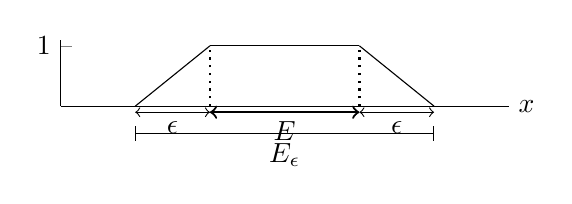
\begin{tikzpicture}
    \begin{axis}[
    axis lines*=left,
    clip = false,
    xmin = 0, xmax = 1, 
    ymin = 0, ymax = 1.1, 
    xtick = \empty, 
    ytick = {1},
    yticklabels={$1$}, 
    axis lines* = left,
    width=0.6\textwidth, height=0.2\textwidth]
    \addplot[domain=1/6:1/3] {6*(x-1/6)};
    \addplot[domain=1/3:2/3] {1};
    \addplot[domain=2/3:5/6] {6*(5/6-x)};
    \addplot[mark=none, black, thick, dotted] coordinates {(1/3,0) (1/3,1)};
    \addplot[mark=none, black, thick, dotted] coordinates {(2/3,0) (2/3,1)};
    \node [right] at (current axis.right of origin){$x$};
    \draw[<->, thick] (1/3, -0.1) to (2/3, -0.1);
    \draw[<->] (1/6, -0.1) to (1/3, -0.1);
    \draw[<->] (2/3, -0.1) to (5/6, -0.1);
    \draw[|-|] (1/6, -0.45) to (5/6, -0.45);
    \node [below] at (1/4, -0.1) {$\epsilon$};
    \node [below] at (3/4, -0.1) {$\epsilon$};
    \node [below] at (1/2, -0.1) {$E$};
    \node [below] at (1/2, -0.45) {$E_\epsilon$};
    \end{axis}
\end{tikzpicture}
    \captionof{figure}{Approximation of an indicator function of a closed-interval.}
\end{center}
Let $E_\epsilon := \set{x \,|\, \rho(x,E) < \epsilon}$. Then clearly 
\begin{equation*}
    \chi_E \leq g_\epsilon \leq \chi_{E_\epsilon} \implies \mu(E) \leq \int_X g_\epsilon(x) \, \mu(dx) = \int_X g_\epsilon(x) \, \nu(dx) \leq \nu(E_\epsilon).
\end{equation*}
But as $\epsilon \searrow 0$ we have $E_\epsilon \searrow E$ and hence by continuity from above we have $\nu(E_\epsilon) \searrow \nu(E)$, so $\mu(E) \leq \nu(E)$. Interchanging $\mu$ and $\nu$ completes the proof.
\end{proof}

As a corollary, 
\begin{corollary}[Uniqueness of weak limit]
If $\mu_n \to \mu$ and $\mu_n \to \nu$ weakly then $\mu = \nu$.
\end{corollary}

\begin{unexaminable}
We may relate the weak convergence of a sequence of measures to functional analysis. This discussion is optional if you have not previously studied functional analysis before, and a good reference would be chapter 3 of \cite{BrezisFuncAnalysis} or section 4.9 of \cite{KreyszigFuncAnalysis}. Recall that $C_b(X)$ is itself a \textbf{Banach} space (i.e. complete normed vector space) equipped with the supremum norm:
\begin{equation}
    \norm{f}_\infty := \norm{f}_{C_b(X)} := \sup_{x \in X} |f(x)|
\end{equation}
We may consider \textbf{functionals} $T: f \mapsto Tf$ that are linear maps from $C_b(X)$ to $\R$. A functional $T$ is bounded (equivalent to being continuous) if there is a constant $C > 0$ such that for all $x$ one have $|Tf(x)| \leq \norm{f}_{C_b(X)}$. The supremum norm now induces a norm on the \textbf{dual space} of $C_b(X)$, i.e. vector space of all bounded linear functional $C_b(X)'$, which is defined as followed:
\begin{equation}
    \norm{T}_{C_b(X)'} := \sup_{f \in C_b(X)} \frac{|Tf|}{\norm{f}_{C_b(X)}} = \inf \set{C>0 \,|\, \forall f \in C_b(X), |Tf| \leq C\norm{f}_{C_b(X)}}.
\end{equation}

\begin{exercise}
Let $\mu$ be a probability measure on $X$. Check that the map 
\begin{equation*}
    T_\mu: f \mapsto \int_X f(x) \, \mu(dx)
\end{equation*}
is a bounded linear functional on $C_b(X)$ with $\norm{T_\mu}_{C_b(X)'} = 1$.
\end{exercise}

We note that there are at least two notions of convergence of functionals in $C_b(X)$: consider functionals $T_n, T \in C_b(X)'$ with $n \in \Z_{\geq 1}$
\begin{itemize}
    \item $T_n \to T$ \textbf{uniformly} if $\norm{T_n - T}_{C_b(X)'} \to 0$ as $n \to \infty$.
    \item $T_n \to T$ \textbf{weakly*} if for all $x \in X$ we have $T_n x \to Tx$. (This corresponds to pointwise convergence).
\end{itemize}

As an important example (which is the point of going through this discussion on this functional analysis topic):
\begin{example}
$\mu_n \to \mu$ weakly $\iff$ $T_{\mu_n} \to T_\mu$ weakly*.
\end{example}

\begin{remark}
Do not be confused with the notion of weak convergence! Weak convergence usually describes the convergence of elements inside a Banach space, not its dual! Of course, one could say that $T_n \to T$ \textbf{weakly} as elements of $C_b(X)'$ as the "intended" Banach space, which refers to $gT_n \to gT$ for all $g$ in the \textbf{double dual} (dual of dual) space $C_b(X)''$. Note that this is strictly stronger than weak* convergence. This is because all evaluation maps $\mathsf{ev}_x: T \mapsto Tx$ are elements in $C_b(X)''$, which means 
\begin{equation*}
    T_n \to T \; \text{weakly} \implies \mathsf{ev}_x T_n = T_n x \to \mathsf{ev}_x T = Tx;
\end{equation*}
but not all elements in $C_b(X)''$ can be represented by the evaluation of an element in $C_b(X)$. In general, the notions of weak and weak* convergence coincide only when we are looking at Banach space for which its double dual coincides with itself.
\end{remark}

We may therefore use the tools from functional analysis to prove theorems relating to weak convergence of measures. For example, we may draw parallels from proposition 3.12 to prove that weakly* convergence induces a topology on the set of probability measures on $(X,\B(X))$, which is generated by neighbourhoods of the following form:
\begin{equation}
    U_{f_1,...,f_k,\epsilon}(\mu) := \set{\nu \,\bigg|\, \forall i = 1,...,k, \abs{\int_X f_i \, \mu(dx) - \int_X f_i \, \nu(dx)} < \epsilon}
\end{equation}
where $\mu, \nu$ is a probability measure on $X$. This also motivates the following definition of the Levy-Prokhorov metric:
\begin{equation}
    \pi(\mu,\nu) := \inf \set{\epsilon > 0 \,|\, \mu(A) \leq \nu(A_\epsilon) + \epsilon \text{ and } \nu(A) \leq \mu(A_\epsilon) + \epsilon},
\end{equation}
where $A_\epsilon := \set{x \,|\, \rho(x,A) < \epsilon}$ is as defined in the proof of lemma \ref{lem:uniqueness_by_integral}. The induced topology is also Polish, which is particularly useful when we want to talk about random probability measures.

\begin{exercise}
Show that for the case when $(X,\B(X)) = (\R,\B(\R))$ then the probability measures $\mu_n \to \mu$ weakly iff $\pi(\mu_n, \mu) \to 0$.  
\end{exercise}

\begin{hint}
Each probability measure of $(\R,\B(\R))$ can be represented by a distribution function. Rewrite the definition of the Levy-Prohorov metric to gain more insights.
\end{hint}
\end{unexaminable}

\subsection{Portmanteau Theorem and related facts}
But wait! We have defined the notion of convergence in distribution in another way in elementary probability classes. Specifically if $(X,\B(X)) = (\R, \B(\R))$ then we say $\xi_n \to \xi$ in distribution if the distribution function $F_{\xi_n}(x) \to F_{\xi}(x)$ for all $x$ when $F_\xi$ is continuous. Turns out the Portmanteau theorem provides us with the required equivalence. This theorem was given its name since it involves a lot of equivalent statements, which look like lots of coats hanging on a coat hanger (\textit{Portmanteau} in French).

\begin{theorem}[Portmanteau Theorem] \label{def:conv_in_dist}
Let $(X,\B(X))$ be a Polish space induced by a metric $d$ and $\mu_n, \mu$ are measures with $\mu_n(X), \mu(X) \leq 1$. Writing $\E_\mu$ as expectation (or integral) with respect to the probability measure $\mu$, then the following are equivalent.
\begin{enumerate}
    \item $\mu_n \to \mu$ weakly, that is, $\forall f \in C_b(X)$, $\E_{\mu_n}[f] \to \E_\mu[f]$.
    \item For all \textbf{uniformly} continuous $f \in C_b(X)$, $\E_{\mu_n}[f] \to \E_\mu[f]$.
    \item For all \textbf{bounded} $f \in \Lip(X)$, $\E_{\mu_n}[f] \to \E_\mu[f]$.
    \item For all bounded measurable $f$ with $\mu(U_f) = 0$, $\E_{\mu_n}[f] \to \E_\mu[f]$, where $U_f$ is the set when $f$ is discontinuous.
    \item $\mu_n(X) \overset{n\to\infty}{\to} \mu(X)$, and for any closed set $E \subseteq X$, $\limsup \mu_n(E) \leq \mu(E)$.
    \item $\mu_n(X) \overset{n\to\infty}{\to} \mu(X)$, and for any open set $O \subseteq X$, $\liminf \mu_n(\xi_n \in O) \ge \mu(\xi \in O)$.
    \item (Convergence in general) $\lim \mu_n (\xi_n \in C) = \mu(\xi \in C)$ for any $C$ such that $\mu(\xi \in \partial C) = 0$.
    % \item Let $F_{\xi_n}(x)$ be the distribution function of $\xi_n$ and similarly for $F_{\xi}(x)$, then $F_{\xi_n}(x) \to F_\xi (x)$ (pointwise) at any point of continuity of $F_\xi(x)$.
\end{enumerate}
\end{theorem}

\begin{figure}
    \centering
    \includegraphics[width=0.5\textwidth]{figures/hanger.jpg}
    \caption{A portmanteau. Figure provided by Hobvias Sudoneighm \url{https://www.flickr.com/people/34427466731@N01} under the Creative Common 2.0 License: \url{https://creativecommons.org/licenses/by-sa/2.0/}}
\end{figure}

\begin{proof} We will follow the order of proving $(4) \implies (1) \implies (2) \implies (3) \implies (5) \implies (6) \implies (7) \implies (4)$. \\

$(4) \implies (1) \implies (2) \implies (3)$. This is trivial.\\

$(3) \implies (5)$. The first condition can be proven by applying (3) with $f \equiv 1$. For the second condition, recall in the proof of lemma \ref{lem:uniqueness_by_integral} we have defined a Lipschitz approximation for any indicator functions of a closed set $E$, which is denoted as $g_\varepsilon(x)$ in equation \eqref{eq:Lipschitz_approx_indicator}. Define also $E_{\varepsilon} = \{ x : \rho(x,E) < \varepsilon\}$. Note that $E_\varepsilon \searrow E$ as $\varepsilon \searrow 0$, so we have
\begin{equation*}
    \mu_n(E) = \int f \, \d \p_n \le \int g_\epsilon \, \d \mu_n.
\end{equation*}
Therefore
\begin{align*}
    \limsup_{n \to \infty} \mu_n(E) \le \limsup_{n \to \infty} \int g_\varepsilon \, \d \mu_n \overset{(3)}{=} \int g_\varepsilon \, \d \mu \leq \mu(E_\varepsilon).
\end{align*}
Since the above inequality holds for all $\epsilon > 0$, we can send $\epsilon \to 0$ to conclude that
\begin{align*}
    \limsup_{n \to \infty} \mu_n(E) \le \mu(E)
\end{align*}
as required. \\

($5 \iff 6$). consider $O = X \backslash E$, $B$ being closed. \\

($5,6 \implies 7$). recall that $\overline{C} = C \cup \partial C$; $C^\circ := \text{int}\, C = C \backslash \partial C$. Since $\p(\xi \in \partial C) = 0$.
\begin{align*}
    &\limsup \mu_n(C) \le \limsup \mu_n (\overline{C}) \overset{(5)}{\le} \mu(\overline{C}) = \mu(C), \\
    &\liminf \mu_n(C) \ge \liminf \mu_n(C^\circ) \overset{(6)}{\ge} \mu(C^\circ) = \mu(C),
\end{align*}
so $\lim \mu_n(C) = \mu(C)$. \\

($7 \implies 4$). Let $f:X \to \R$ be a bounded and measurable function with $\mu(U_f) = 0$. We make the following claims:\\

\textbf{Claim 1:} For all $D \subseteq \R$, $\partial f^{-1}(D) \subseteq f^{-1}(\partial D) \cup U_f$.

\begin{hint}
What happen if $x \in \partial f^{-1}(D)$ but $x \notin U_f$, i.e. $f$ is continuous at $x \in E$? Recall the definition of continuity at $x \in E$: $\forall \epsilon > 0,\; \exists \delta := \delta(\epsilon) > 0$ such that $f(B_\delta(x)) \subseteq B_\epsilon(f(x))$. Also recall that $f(x) \in \partial D$ iff $\forall \epsilon > 0$, $B_\epsilon(D) \cap A \neq \varnothing$ and $B_\epsilon(D) \cap A^c \neq \varnothing$.
\end{hint}

\textit{Proof of claim 1.} Fix $\epsilon>0$ and extract $\delta := \delta(\epsilon)$ as above. Provided that $x \in \partial f^{-1}(D)$, we know that there is a $y \in B_\delta(x) \cap f^{-1}(D)$ and $z \in B_\delta(x) \cap X\setminus f^{-1}(D)$. We therefore have
\begin{align*}
    f(y) \in f(B_\delta(x) \cap f^{-1}(D)) \subseteq f(B_\delta(x)) \cap f(f^{-1}(D)) \subseteq B_\epsilon(f(x)) \cap D 
\end{align*}
and similarly $f(z) \in B_\epsilon(f(x)) \cap D^c$. Since $\epsilon > 0$ is arbitrary we have $f(x) \in \partial D$ as desired. \\

\textbf{Claim 2:} Consider the set $A := \set{y \in \R \,|\, \mu(f(x) = y) > 0}$, i.e. set of atoms of the finite push-forward measure $f^*\mu$. Then $A$ must be countable.\\

We leave that as an exercise.\\

\textit{Finishing the proof.} Fix $\epsilon > 0$ and let $\norm{f}_\infty = \sup_{x\in X} |f(x)|$ (for the case when $f$ is continuous then $\norm{f}_\infty$ coincides with $\norm{f}_{C_b(X)}$).  Then by claim 2, we may choose $N+1$ "grid points" such that 
\begin{equation*}
    y_0 \leq -\norm{f}_\infty < y_1 < ... < y_{N-1} < \norm{f}_\infty < y_N,
\end{equation*}
such that for all $i$,
\begin{equation*}
    y_i \in \R \setminus A \quad \text{and} \quad y_{i+1} - y_i < \epsilon.
\end{equation*}

Now let $X_i = f^{-1}([y_{i-1}, y_i))$ for $i=1,...,N$. Then $X = \sqcup_{i=1}^N X_i$. By claim 1, we have
\begin{equation*}
    \mu(\partial X_i) \leq \mu(f^{-1}(\set{y_{i-1}})) + \mu(f^{-1}(\set{y_{i}})) + \mu(U_f) = 0
\end{equation*}

Therefore,
\begin{align*}
    \limsup_{n\to\infty} \int f \, \mu_n(dx) \leq \limsup_{n\to\infty} \sum_{i=1}^N y_i \mu_n(E_i) \overset{(7)}{=} \sum_{i=1}^N y_i \mu(E_i) \leq \epsilon \mu(X) + \sum_{i=1}^N y_{i-1} \mu(E_i) \leq \varepsilon + \int f \, \mu(dx)
\end{align*}

Since the above arguments hold for arbitrary $\epsilon > 0$, we see that 
\begin{equation*}
\limsup_{n\to\infty} \int f \, \mu_n(dx) \leq \int f \, \mu(dx)
\end{equation*}
We complete the proof by applying the above inequality with $-f$ to obtain the reverse inequality:
\begin{equation*}
\limsup_{n\to\infty} \int -f \, \mu_n(dx) \leq \int -f \, \mu(dx) \iff \int f \, \mu(dx) \leq \liminf_{n\to\infty} \int f \, \mu_n(dx)
\end{equation*}
\end{proof}

\begin{exercise}
\begin{enumerate}
    \item[]
    \item Rewrite the statements of Portmanteau theorem for a sequence of random variables that converge in distribution.
    \item Fill in the gap: prove that there are at most countable atoms for the finite measure $f^*\mu$.
\end{enumerate}
\end{exercise}

\begin{hint}
Argue by contradiction. The key step is to convince yourself that if $A$ is uncountable then there is an $\epsilon > 0$ such that $f^*\mu((\set{x})) \geq \epsilon$ for uncountably many $x \in A$ (otherwise you will have $A$ being countable!)
\end{hint}

We now look at some applications of the Portmanteau theorem:
\subsubsection{Slutsky's Theorem and Convergence of Probability}
Slutsky's theorem is the core of establishing the fact that convergence in probability implies convergence in distribution, as well as a couple of other facts relating to the arithmetic of weak limits of converging sequence of random variables. Let us now go through the statement of Slutsky's theorem:

\begin{theorem}[Slutsky]
Consider random variables $\xi, \xi_1,...$ and $\eta,\eta_1,...$ from $(\Omega,\F,\p)$ to the Polish space $(X,\B(X))$ with metric $d$. Assume $\xi_n \overset{n\to\infty}{\to} \xi$ in distribution and $d(\xi_n, \eta_n) \overset{n\to\infty}{\to} 0$ in probability. Then $\eta_n \overset{n\to\infty}{\to} \xi$ in distribution.
\end{theorem}

\begin{proof}
Let $f:X \to \R$ be a bounded and Lipschitz function $f \in \Lip_{K}(X)$. Then for all $x \in E$,
\begin{equation}
    \abs{f(x) - f(y)} \leq Kd(x,y) \wedge 2\norm{f}_{C_b(X)}.
\end{equation}
So by dominated convergence theorem one have $\limsup_{n\to\infty} \E_{\p}[|f(\xi_n) - f(\eta_n)|] = 0$. But we also have $\limsup_{n\to\infty} \E_{\p}[|f(\xi_n) - f(\xi)|] = 0$ by convergence in probability, so combining yields $\limsup_{n\to\infty} \E_{\p}[|f(\eta_n) - f(\xi)|] = 0$. By statement (3) of the Portmanteau theorem we have $\eta_n \overset{n\to\infty}{\to} \xi$ in distribution.
\end{proof}

As an immediate corollary:
\begin{corollary} \label{cor:prob_implies_dist}
Let $\xi_n, \xi: (\Omega,\F,\p) \to (X,\B(X))$, then $\xi_n \overset{n\to\infty}{\to} \xi$ in probability implies $\xi_n \overset{n\to\infty}{\to} \xi$ in distribution. Moreover if $\xi_n \overset{d}{\to} \xi$ and $\xi \equiv c$ for some constant $c$, then $\xi_n \overset{p}{\to} c$.
\begin{figure} [H]
    \centering
    \begin{tikzcd}
    & \overset{L^p}{\to} \arrow[Rightarrow, d]  & \\
    \overset{a.e.}{\to} \arrow[Rightarrow, r] & \textcolor{red}{\overset{p}{\to}} \arrow[Rightarrow, r, red] & \textcolor{red}{\overset{d}{\to}}
\end{tikzcd}
\end{figure}
\end{corollary}

\begin{proof} 
First statement is proven by applying $\xi_n \equiv \xi$. As for the second statement, let's say $\xi_n \overset{d}{\to} c$ where $c$ is a constant. Then by utilising statement (5) of the Portmanteau theorem, we know that
\begin{equation*}
    \lim_{n\to \infty} \p(d(\xi_n, c) \geq \epsilon) = \lim_{n\to \infty} \p(\xi_n \in X \setminus B_\epsilon(c)) \leq \p(c \in X \setminus B_\epsilon(c)) = 0.
\end{equation*}
\end{proof}

\begin{remark}
\begin{itemize}
\item[]
\item An alternative proof of the partial converse is as followed: if we assume the metric form of convergence in probability, then we can directly write 
\begin{equation}
    \E[d(X_n, c) \wedge 1] \overset{n\to\infty}{\to} 0,
\end{equation}
noticing that the function $f(.) = d(.,c) \wedge 1$ is a continuous and bounded function on $X$.
\item A counter-example showing convergence in distribution does not imply convergence in probability is as followed: consider a real-valued random variable $X$ that is symmetric about zero, e.g. $\xi \sim \mathsf{N}(0,1)$. Then the sequence $\xi_n := (-1)^{n+1}\xi$ converges in distribution (since they are identically distributed) but not in probability.
\end{itemize}
\end{remark}

Here is an example of using the above implication. 
\begin{example}[Motivation of Weierstrass Approximation Theorem]
Recall the Bernoulli's law of large numbers, that for all $p \in [0,1]$,
\begin{equation*}
    \frac{S_n}{n} \xrightarrow{p} p, \quad n \to \infty,
\end{equation*}
where $S_n = \xi_1 + \xi_2 + \cdots + \xi_n$ and $\xi_i \sim \mathsf{B}(1,p)$. Putting
\begin{equation*}
    F_n(x) = \p \bigg(\frac{S_n}{n} \le p \bigg), \quad F(x) = 
    \begin{cases}
    1, & x \ge p,\\
    0, & x<p,
    \end{cases}
\end{equation*}
where $F(x)$ is the distribution function of the constant random variable $\xi \equiv p$. Also let $\p_n$ and $\p$ be the probability measures on $(\R, \B(\R))$ corresponding to the distributions $F_n, F$. The above implication implies that $S_n/n \xrightarrow{d} p$, which means from statement (1) that
\begin{equation*}
    \E\bigg[f\bigg(\frac{S_n}{n} \bigg) \bigg] \to \E[f(p)] = f(p), \quad n \to \infty,
\end{equation*}
for every bounded function $f(x) \in C_b(\R)$. Since $S_n \sim \mathsf{B}(n,p)$, we know that
\begin{equation*}
    \E\bigg[f\bigg(\frac{S_n}{n} \bigg) \bigg] = \int_\R f(x) \, \p_n(\d x) = \sum_{k=0}^n \sqbracket{{n \choose k}(1-p)^{n-k} p^k} f\bracket{\frac{k}{n}} =: f_n(p)
\end{equation*}
which is a polynomial in $p$. We therefore have for all $f \in C_b(\R)$, $f_n(p) \to f(p)$ pointwise for all $p \in [0,1]$. Restricting $f$ to the compact interval $[0,1]$, we have recovered a weakened version of the Weierstrass approximation theorem, that there is a sequence of polynomials $f_n$ such that $f_n \to f$ pointwise on $[0,1]$. The actual approximation theorem goes further and establishes that the above convergence is actually uniform on $[0,1]$.
\end{example}

Here is another application of Slutsky's theorem regarding the addition of weak limits. This result is also named after Slutsky due to its relation with the original Slutsky's theorem.
\begin{proposition}[Slutsky, Addition of Limits] \label{prop:addition_of_weak_limits}
Consider random variables $\xi, \xi_1,...$ and $\eta_1,...$ from $(\Omega,\F,\p)$ to $(\R,\B(\R))$ (or any Polish space with addition defined). Assume $\xi_n \overset{n\to\infty}{\to} \xi$ in distribution and $\eta_n \overset{n\to\infty}{\to} c$ in probability, with $c$ being a constant. Then $\xi_n + \eta_n \overset{n\to\infty}{\to} \xi + c$ in distribution.
\end{proposition}

\begin{proof}
First it is easily to check by that $\xi_n + c \overset{n\to\infty}{\to} \xi_n + c$ in distribution. (This can be done by e.g. shifting the closed sets and applying statement (5) of the Portmanteau theorem. Now note that $|(\xi_n + \eta_n) - (\xi_n + c)| \overset{n\to\infty}\to 0$ in probability, so by Slutsky's theorem we have $\xi_n + \eta_n \to \xi_n + c$ in distribution.
\end{proof}

Note that it is not true in general that both $\xi_n \overset{n\to\infty}\to \xi$ and $\eta_n \overset{n\to\infty}\to \eta$ in distribution implies $\xi_n + \eta_n \overset{n\to\infty}\to \xi + \eta$ in distribution. As an example, consider again the real-valued random variable $\xi$ that is symmetric about zero. If $\xi_n \equiv \xi$ and $\eta_n = (-1)^{n+1} \xi$, then $\xi_n + \eta_n$ takes the form $(2\xi, 0, 2\xi, 0, ...)$ which does not converge in distribution.\\

Traditionally, Slutsky's theorem also contains the following statements
\begin{proposition}[Slutsky, Multiplication/Division of Limits] \label{prop:mult_of_weak_limits}
Under the same setting as proposition \ref{prop:addition_of_weak_limits}, we have $\xi_n \eta_n \overset{n\to\infty}{\to} c\xi$ in distribution. In addition if $c \neq 0$ then $\xi_n / \eta_n \overset{n\to\infty}{\to} \xi / c$.
\end{proposition}

To prove this, we note the following result:
\begin{proposition}[Continuous Mapping Theorem] 
Let $(X_1,\B(X_1))$ and $(X_2,\B(X_2))$ be metric spaces generated by metric $d_1$ and $d_2$ respectively, and let $\varphi: X_1 \to X_2$ be measurable. If $U_\varphi$ is the set of points of discontinuity of $\varphi$ (which is Borel measurable), then
\begin{enumerate}
\item If $\mu, \mu_1, \mu_2, ...$ are measures on $(X_1,\B(X_1))$ with $\mu(X_1), \mu_n(X_1) \leq 1$ and $\mu(U_\varphi) = 0$ and $\mu_n \overset{n\to\infty}\to \mu$ weakly, then $\varphi^*\mu_n \overset{n\to\infty}{\to} \varphi^*\mu$ weakly.
\item If $\xi, \xi_1, \xi_2, ...: (\Omega,\F,\p) \to (X_1, \B(X_1))$ are random variables with $\p(\xi \in U_\varphi) = 0$ and $\xi_n \overset{n\to\infty}\to \xi$ in distribution, then $\varphi(\xi_n) \overset{n\to\infty}\to \varphi(\xi)$
\end{enumerate}
\end{proposition}

\begin{proof}
Note that the second statement is an immediate result of the first one. To prove the first statement, we are required to show that for all $f \in C_b(X_2)$,
\begin{align*}
    \lim_{n\to\infty} \int_{X_2} f(x_2) \,\varphi^*\mu_n(dx_2) &\overset{\text{(LOTUS)}}{=} \lim_{n\to\infty} \int_{X_1} f(\varphi(x_1)) \,\mu_n(dx_1) \\
    &\overset{(*)}{=} \int_{X_1} f(\varphi(x_1)) \,\mu(dx_1) \\
    &\overset{\text{(LOTUS)}}{=} \int_{X_2} f(x_2) \, \varphi^*\mu(dx_1).
\end{align*}
The first and third equality is justified by the use of the change of variable formula (theorem \ref{thm:LOTUS}). The second equality is justified by noting that $U_{f \circ \varphi} \subseteq U_\varphi$, so $\mu(U_{f \circ \varphi}) = 0$ and we may use statement (4) of the Portmanteau theorem to conclude.
\end{proof}

We also note the following:
\begin{exercise}
Under the setting of proposition \ref{prop:addition_of_weak_limits}, consider the random variables $T_n: \omega \in \Omega \mapsto (\xi_n(\omega), \eta_n(\omega))$ and $T: \omega \in \Omega \mapsto (\xi_n(\omega), c)$. Then $T, T_n$ are $(\R^2, \B(\R^2))$-valued random variables. Show that $T_n \overset{n\to\infty}\to T$ in distribution. 
\end{exercise}

\begin{hint}
Try mimick the proof of proposition \ref{prop:addition_of_weak_limits} by proving that $(X_n, c) \overset{n\to\infty}{\to} (X_n, c)$ in distribution and $|(X_n, Y_n) - (X_n, c)| \overset{n\to\infty}{\to} 0$ in probability, then utilise Slutsky's theorem.
\end{hint}

\begin{proof}
\textit{of proposition \ref{prop:addition_of_weak_limits}/\ref{prop:mult_of_weak_limits}.} Apply the result in the above exercise and continuous mapping theorem with map $\varphi(x,y) = x+y$, $xy$ or $x/y$.
\end{proof}

\subsubsection{Convergence of distribution function}
Let us finally connect our definition of weak convergence with the definition of convergence of distribution in elementary probability classes, that is, the convergence of the distribution function. We restrict our discussion to real-valued random variables, although it can be extended to random variables taking value on $\R^n$.

\begin{theorem}[Convergence in distribution] \label{thm:conv_in_dist_func}
\begin{enumerate}
\item[]
\item Consider measures $\mu, \mu_n$ on $(\R,\B(\R))$ with $\mu(\R), \mu_n(\R) \leq 1$ and define their distribution functions $F(x) := \mu((-\infty,x])$ and $F_n(x) := \mu_n((-\infty, x])$. Then $\mu_n \overset{n\to\infty}{\to} \mu$ weakly $\iff$ 
\begin{itemize}
\item $F_n(x) \overset{n\to\infty}\to F(x)$ for all $x \in \R \setminus U_F$, $U_F$ being the set of discontinuities of $F$, and 
\item $F_n(+\infty) \to F(+\infty) =: \lim_{x\to +\infty} F(x)$. 
\end{itemize}

\item Consider random variables $\xi_n, \xi : (\Omega,\F,\p) \to (\R,\B(\R))$, then $\xi_n \overset{n\to\infty}{\to} \xi$ in distribution $\iff$ 
\begin{itemize}
\item $F_{\xi_n}(x) \overset{n\to\infty}{\to} F_\xi(x)$ when $x \in \R \setminus U_{F_\xi}$.
\item $F_{\xi_n}(+\infty) \overset{n\to\infty}{\to} F_\xi(+\infty)$
\end{itemize}
\end{enumerate}
\end{theorem}

\begin{remark} \label{rmk:weakening_conv_in_dist}
We note that convergence at all points of continuity implies 
\begin{equation}
F(+\infty) \leq \liminf_{n\to\infty} F_{n}(+\infty)
\end{equation}
To see this, we note that for all $x$, we have $F(x) \leq \liminf_{n\to\infty} F_n(+\infty)$. Fix an $x \in \R$, then there is an $r > x$ such that $F$ is continuous at $r$. At this point we have $\liminf_{n\to\infty} F_n(r) = \lim_{n\to\infty} F_n(r) = F(r)$. Now note that, for all $n$, $F_n(r) \leq F_n(+\infty)$, so we have $F(x) \leq \liminf_{n\to\infty} F_{n}(+\infty)$. Since $x$ is arbitrary, we know that $F(+\infty) \leq \liminf_{n\to\infty} F_{n}(+\infty)$.\\

From this, we know that if $F(+\infty) \geq \limsup_{n\to\infty} F_n(+\infty)$, then $\mu_n \overset{n\to\infty}{\to} \mu$ weakly.
\end{remark}

\begin{proof}
We note that statement (2) immediately follows from (1). For the $(\Rightarrow)$ direction, it follows from the fact that $\mu(\partial (-\infty, x]) = \mu(\set{x}) = 0$ whenever $F$ is continuous at $x$, so by statement (7) of Portmanteau theorem we have $F_n(x) \overset{n\to\infty}{\to} F(x)$. For the $(\Leftarrow)$ direction, we attempt to use statement (3) of the Portmanteau theorem; that is, if $f$ is a bounded Lipschitz function (wlog $f \in \Lip_1(\R)$ and bounded by $1$), then
\begin{equation*}
    \lim_{n\to\infty} \int_\R f(x) \, \mu_n(dx) = \int_\R f(x) \, \mu(dx).
\end{equation*}
Using arguments in proving $(7) \implies (4)$ in the Portmanteau theorem, we know that $U_F$ is countable. As a result, we may choose $N$ "knot points", but in a way different from the one in the proof of the Portmanteau theorem. Specifically, we want
\begin{equation*}
    y_1 < y_2 < ... < y_{N-1}
\end{equation*}
such that for all $i$,
\begin{equation*}
    y_i \notin U_F, \quad y_i - y_{i-1} < \epsilon, \quad F(y_1) < \epsilon, \quad F(y_{N-1}) > F(\infty) - \epsilon.
\end{equation*}
With the notation of $y_0 = -\infty$ and $y_N = \infty$ (so that $F(y_0)=F_n(y_0)=0$), we obtain the bound:
\begin{align*}
    \int f(x) \, \mu_n(dx) = \sum_{i=0}^n f(x) \, \mu_n(dx) &\leq F_n(y_1) + F_n(\infty) - F_n(y_{N-1}) + \sum_{i=1}^{N-1} \int_{y_i}^{y_{i+1}} f(x) \, \mu_n(dx).
\end{align*}
But we know that for all $x \in [y_i, y_{i+1})$ 
\begin{equation*}
    |f(x) - f(y_i)| \leq |x-y_i| \leq y_i - y_{i-1} < \epsilon \implies f(y_i) - \epsilon < f(x) < f(y_i) + \epsilon,
\end{equation*}
so
\begin{align*}
    \int f(x) \, \mu_n(dx) &< \bracket{F_n(y_1) + F_n(\infty) - F_n(y_{N-1})} + \sum_{i=1}^{N-1} (f(y_i) + \epsilon)(F_n(y_{i+1}) - F_n(y_{i})) \\
    &= \bracket{F_n(y_1) + F_n(\infty) - F_n(y_{N-1})} + \sum_{i=1}^{N-1} f(y_i)(F_n(y_{i+1}) - F_n(y_{i})) + \epsilon F_n(\infty)
\end{align*}
Note that for all $i$, $F_n(y_i) \overset{n\to\infty}{\to} F(y_i)$. Recall that $F(\infty) \leq 1$, we have
\begin{align*}
    \limsup_{n\to\infty} \int f(x) \, \mu_n(dx) &< 3\epsilon + \sum_{i=1}^{N-1} f(y_i)(F(y_{i+1}) - F(y_{i})) \\
    &\leq \int_{i=1}^{N-1} \int_{y_i}^{y_{i+1}} (f(x)+\epsilon) \, \mu(dx) \\
    &\leq 4\epsilon + \int f(x) \, \mu(dx)
\end{align*}
owing to the fact that $f(x) + \epsilon \geq f(y_i)$ for all $x \in [y_i, y_{i+1})$. Sending $\epsilon \searrow 0$ yields
\begin{align*}
    \limsup_{n\to\infty} \int f(x) \, \mu_n(dx) \leq \int f(x) \, \mu(dx)
\end{align*}
Replacing $f$ by $(1-f)$ yields the desired reverse inequality.
\end{proof}

Here we raise some applications of the above result. First of all, (theorem \ref{thm:deMoivre_CLT})
\begin{example}[de Moivre's Central Limit Theorem] \label{ex:deMoivre_CLT_conv_dist}
For $\xi_i \overset{\mathsf{iid}}{\sim} \mathsf{B}(1,p)$ and $S_n = \sum_{i=1}^n \xi_i$, recall the random variable $\eta_n = (S_n-np)/\sqrt{np(1-p)}$ satisfies
\begin{equation*}
    \lim_{n \rightarrow \infty} \p (\eta_n \le x) = \Phi (x),
\end{equation*}
where $\Phi(x)$ is the distribution function of the standard normal $\mathsf{N}(0,1)$ distribution. Therefore, \textbf{the probability distribution of $\eta_n$ converges to a $\mathsf{N}(0,1)$ distribution}. By definition of weak convergence, for any $f \in C_b(\R)$ we know that
\begin{equation}
\E\sqbracket{f\bracket{\frac{S_n-np}{\sqrt{np(1-p)}}}} \overset{n\to\infty}{\to} \int_\R f(t) \bracket{\frac{1}{\sqrt{2\pi}} e^{-t^2/2}} \, dt
\end{equation}
\end{example}

Here is another shortcut for proving convergence in distribution via the convergence of their densities.

\begin{corollary}
Suppose that the random variables $\xi_n, \xi$ have densities $f_n(x), f(x)$, respectively. Also let $f_n(x) \to f(x)$ for any $x$. Then $\xi_n \xrightarrow{d} \xi$.
\end{corollary}

\begin{proof}
It is sufficient to show that 
\begin{equation*}
    F_n(x) = \int_{-\infty}^x f_n(y) \, \d y \to F(x) = \int_{-\infty}^x f(y) \, \d y
\end{equation*}
for any $x$. Using 
\begin{equation*}
    |F_n(x) - F(x)| \le \int_{-\infty}^x |f_n(y) - f(y)| \, \d y,
\end{equation*}
we need to check that
\begin{equation*}
    \lim_{n \to \infty} \int_{-\infty}^\infty |f_n(y) - f(y)| \, \d y = 0.
\end{equation*}
Note that $a = a_+ - a_-$ and $|a| = a_+ + a_-$ for any real $a$. Since $f_n$ and $f$ are densities, they integrate to $1$, so for each $n$
\begin{equation*}
    0 = \int_{-\infty}^\infty (f(y) - f_n(y)) \, \d y = \int_{-\infty}^\infty [(f(y) - f_n(y))_+ - (f(y) - f_n(y))_-] \, \d y.
\end{equation*}
Then
\begin{equation*}
    \int_{-\infty}^\infty |f(y) - f_n(y)| \, \d y = 2\int_{\infty}^\infty(f(y) - f_n(y))_+ \, \d y,
\end{equation*}
which goes to zero by the dominated convergence theorem. Indeed 
\begin{equation*}
    0 \le (f(y) - f_n(y))_+ \le f(y),
\end{equation*}
for any $n$ and the function $f(y)$ is integrable.
\end{proof}

\begin{exercise}[Uniform convergence of distribution function] \label{ex:uniform_conv_of_dist}
\begin{enumerate}
    \item[]
    \item Let $F_n \to F$ and suppose that $F$ is continuous. Show that $F_n$ converges \textit{uniformly} to $F$, i.e.
    \begin{equation*}
        \sup_x |F_n(x) - F(x)| \to 0, \quad n \to \infty.
    \end{equation*}
    \textit{Hint:} Idea is to consider knot points as in theorem \ref{thm:conv_in_dist_func}.
    \item Give an example of distribution functions $F_n(x), F(x)$ such that $F_n(x) \xrightarrow{d} F(x)$, but 
    \begin{equation*}
        \sup_x |F_n(x) - F(x)| \not \to 0, \quad n \to \infty.
    \end{equation*}
    \item Give an example of probability measures $\p, \p_n$ on $(\R, \B(\R))$, $n \ge 1$ such that $\p_n \xrightarrow{d} \p$, but convergence $\p_n(B) \to \p(B)$ need not hold for all Borel sets $B \in \B(\R)$.
\end{enumerate}
\end{exercise}

\subsection{Skorohod Representation Theorem}
We now prove that a sequence of weakly convergence probability measures can be represented as random variables defined on a common probability space.

\begin{theorem}[Skorohod Representation Theorem]
Suppose $\mu, \mu_n \, (n=1,2,...)$ are probability measures on a Polish space $(X,\B(X))$ induced by a metric $d$, so that $\mu_n \overset{n\to \infty}{\to} \mu$ weakly. Then there exists a single probability space $(\Omega', \F', \p')$ and random variables $\xi_1, \xi_2, \dots$ on it such that $\xi$ has distribution $\mu$ ($\xi^*\p = \mu$), $\xi_n$ has distribution $\mu_n$ ($\xi_n^*\p = \mu_n$) and that $\xi_n \to \xi$ $\p$-almost surely.
\end{theorem}

We will not go through the proof for general Polish space, if interested one can read Dudley's paper \cite{DudleySkorohod}. However if we limit ourselves to the case when $(X,\B(X)) = (\R, \B(\R)))$ then there is a simple proof.

\begin{proof}
Let $(\Omega',\F',\p') = ([0,1], \B([0,1], \Leb))$. Note that the probability measures $\mu, \mu_n$ induces distribution functions $F_n, F: \R \to [0,1]$. Let $F^{-1}, F_n^{-1}$ be their right inverses as defined in equation \ref{eq:right_inverse}, then by probability integral transform (proposition \ref{prop:prob_transform}), they have same distribution as $\mu$ and $\mu_n$'s respectively. It remains to prove that $F_n^{-1}(u) \to F^{-1}(u)$ almost surely as $n \to \infty$. In fact we can prove the required limit for any $u$ such that the preimage of $\set{u}$ under $F$ is finite (i.e. a singleton or empty set). Since there are only countably many $u$ such that the above condition doesn't hold (given that $F$ is increasing and right continuous), establishing the above limit will complete the proof. \\

Let $u$ be a point such that the preimage of $\set{u}$ under $F$ is finite. We make two observations:
\begin{itemize}
\item If $x < F^{-1}(u)$, then using the argument in the proof of proposition \ref{prop:prob_transform} we have $F(x) < u$. If $F$ is continuous at $x$, then by extending the arguments in the above proof of Portmanteau theorem we see that $F_n(x) \to F_\xi(x)$ as $n \to \infty$, and that for sufficiently large $n$ we have $F_n(x) < u \iff x \leq F_n^{-1}(u)$. We therefore have $x \leq \liminf_{n\to\infty} F_n^{-1}(u)$. Now consider a sequence $x_k \nearrow F^{-1}(u)$ such that $F$ is continuous as $x_k$, which exists by the fact that $F$ is increasing (otherwise $F$ have uncountable discontinuities!) Then for all $k$ one have $x_k \leq \liminf_{n\to\infty} F_n^{-1}(u)$, and that $F^{-1}(u) \leq \liminf_{n\to\infty} F_n^{-1}(u)$ by sending $k \to \infty$.
\item If $x > F^{-1}(u)$, then $F(x) \geq u$. In fact we must have $F(x) > u$, for if $F(x) = u$ then $F(y) = u$ for any $y \in [F^{-1}(u), x]$, contradicting the assumption that the preimage of singleton $\set{u}$ is finite. Repeating the above arguments yields $F^{-1}(u) \geq \limsup_{n\to\infty} F_n^{-1}(u)$.
\end{itemize}
Combining the observations we have $F_n^{-1}(u) \to F^{-1}(u)$ as desired.
\end{proof}

As a result, we may restate any theorems (including Central Limit Theorem) in terms of random variables.
\begin{example}[Restating de Moivre's CLT]
We may construct a probability space $(\Omega, \F, \p)$, random variables $\eta_n, \eta$ such that $\eta$ is normally distributed and $\sqrt{np(1-p)}\eta_n + np$ has a $\mathsf{B}(n,p)$ distribution. 
\end{example}

Of course, more effort is needed to actually construct a probability space $(\Omega, \F, \p)$, random variables $\xi_n \overset{\text{iid}}\sim \mathsf{B}(1,p)$ and $\eta \sim \mathsf{N}(0,1)$ such that the de Moivre's CLT holds, and this will be omitted in our discussion. Nevertheless, this representation theorem gives us a shortcut for proving results relating to the weak convergence.

\begin{example}[Alternative proof of the theorem \ref{thm:conv_in_dist_func}]
Let's say we have probability measures $\p_n, \p$ on $(\R,\B(\R))$ such that their distribution function converges at all points of continuity. By Skorohod representation theorem, we may construct a sequence of random variables $\bar{\xi}, \bar{\xi}_1, \bar{\xi}_2,...$ on the common probability space $([0,1], \B([0,1]), \Leb)$ with distributions $F_\xi, F_{\xi_1}, F_{\xi_2}, ...$. Let $f \in C_b(\R)$, then by change of variable and dominated (or bounded) convergence theorem, 
\begin{equation*}
    \lim \E_{\p_n} [f_n(\xi_n)] = \lim \E_{\Leb} [f_n(\bar{\xi}_n)] \overset{\text{(DCT)}}{=} \E_{\Leb}[f(\bar{\xi})] = \E_{\p}[f(\xi)],
\end{equation*}
noting that $f_n(\bar{\xi}_n) \to f_n(\bar{\xi})$ almost surely (convince yourself!) This completes the proof.
\end{example}

\subsection{Relative Compactness and Tightness}
We will later prove the well-known Central Limit Theorem by looking at characteristic functions. To establish the relationship between characteristic functions and measures, we need some tools relating to the collections of measures, including clarifying the meaning of how a collection is \textit{relatively compact} and \textit{tight}. These concepts are also very useful in proving results relating to stochastic processes and ergodic theory. We begin by the following definition:

\begin{definition}
A family of probability measures $\mathcal{P} = \{ \p_\alpha, \alpha \in A\}$ on a Polish space (and the corresponding set of distribution functions $F_\alpha$ if the underlying Polish space is $(\R^n, \B(\R^n))$) is called \textbf{relatively compact} if every sequence of measures from $\mathcal{P}$ contains a subsequence that weakly converges to a probability measure.
\end{definition}

\begin{remark}
We emphasise that in this definition the limit measure is to be a probability measure, although it need not belong to the original class $\mathcal{P}$. (This is why the word “relatively” appears in the definition.) In fact, $\mathcal{P}$ is relatively compact if its closure with respect to the Levi-Prokhorov metric is compact.
\end{remark}

As an example, the collection containing a weakly convergent sequence of measures is relatively compact. In fact, we have the following.
\begin{lemma} \label{lem:weak_conv_further_subsequence}
If $\{\p_{n}\}$ and $\p$ are probability measures, then $\p_n \xrightarrow{d} \p$ if and only if every subsequence $\{\p_{n'}\}$ of $\{\p_{n}\}$ contains a subsequence $\{\p_{n''}\}$ such that $\p_{n''} \xrightarrow{d}\p$.
\end{lemma}
\begin{proof}
From the definition of weak convergence we know that $\p_n \xrightarrow{d}\p$ if and only if the following sequence of numbers converges for any continuous bounded function $f$:
\begin{equation*}
    \int f(x) \, \p_n(\d x) \to \int f(x) \, \p (\d x).
\end{equation*}
So necessity is trivial, just take $\{n''\}=\{n'\}$. For the sufficiency, assume the converse to get a contradiction. Then there exists an $f$, an $\varepsilon>0$ and a subsequence $\{n'\}$ such that 
\begin{equation*}
    \bigg|\int f(x) \p_{n'}(\d x) - \int f \, \p(\d x) \bigg| > \varepsilon \quad \forall n'.
\end{equation*}
This clearly can not be true as by the assumption, $\p_{n''} \xrightarrow{d} \p$, so 
\begin{equation*}
    \bigg|\int f(x) \p_{n'}(\d x) - \int f \, \p (\d x) \bigg| < \varepsilon
\end{equation*}
for large enough $n''$.
\end{proof}

A given family of probability measures $\mathcal{P}$ is not necessarily relatively compact. This is illustrated by the following examples.
\begin{example} \label{ex:limits_not_a_distribution}
Let $\xi_n$ be real-valued random variables and $F_{\xi_n}(x) \to F(x)$ for all $x \in U_F$. Then $F(x)$ is not necessarily a distribution function!
\begin{enumerate}
    \item Let $\xi_n$ be $U[n, n+1]$. Then $F(x) \equiv 0$ (called runaway to infinity).
    \item Let $\xi_n$ be $U[-n, n]$. Then $F(x) \equiv 1/2$ (called spread to infinity).
\end{enumerate}
\end{example}

The following theorem will provide a necessary and sufficient condition for a family of probability measures (or finite measures) to be relatively compact. We first define the notion of tightness:
\begin{definition}[Tightness] \label{def:tightness}
A family of probability measures $\mathcal{P} = \{ \p_\alpha\}_{\alpha \in A}$ on a Polish space $(X, \B(X))$ induced by metric $d$ (or family of finite measures $\set{\mu_\alpha}_{\alpha \in A}$ with $\mu_\alpha(X) \leq 1$) is \textbf{tight} if for all $\varepsilon>0$ there exists a compact set $K \subset X$ such that
\begin{equation}
    \sup_{\alpha \in A} \p_\alpha (X \backslash K) \le \varepsilon.
\end{equation}
\end{definition}

Turns out tightness is a sufficient condition for relative compactness (and is necessary if $(X,\B(X))$ is Polish)
\begin{theorem}[Prokhorov's theorem]
A tight family of probability measures $\mathcal{P}$ (or finite measures as specified in definition \ref{def:tightness}) of $(X,\B(X))$ induced by metric is relatively compact. If in addition $(X,\B(X))$ is Polish then the converse also holds.
\end{theorem}

Here we only discuss the proof for the case when $(X,\B(X)) = (\R,\B(\R))$. In such case, the Prokhorov's theorem reduces to the Helly's selection theorem. We denote the collection of functions $\mathcal{G} = \{ F: \R \to [0,1] \}$ such that $F$ is nondecreasing, continuous from the right. This is called the set of generalised distribution functions. 

\begin{remark}
Distribution functions form a subset of $\mathcal{G}$ for which $F(-\infty) = 0$ and $F(\infty) = 1$.
\end{remark}

We may then state the Helly's theorem
\begin{theorem}[Helly's Selection Theorem] \label{thm:Helly_selection}
The set $\mathcal{G}$ of generalised distribution functions is sequentially compact, i.e. for any sequence $F_n \in \mathcal{G},$ $n=1,2,\dots$ there exists a function $F \in \mathcal{G}$ and a subsequence $F_{n_k} \subseteq \{ F_n\}$ such that $F_{n_k}(x) \to F(x)$ for every point $x \in \R \setminus U_F$, $U_F$ being set of points of discontinuities of $F$.
\end{theorem}

\begin{proof}
The theorem uses a classic diagonal sequence argument. Let $(q_k)_{k\geq 1}$ be an enumeration of $\Q$ (bijection from $\N$ to $\Z$). 
\begin{itemize}
\item Consider the sequence $(F_n(q_1))_{n\geq 1}$, which is bounded, so by Bolzano-Weierstrass theorem (BW) it has a subsequence $\bracket{F_{n_k^{(1)}}(q_1)}_{k \geq 1}$ which converges to some number $G(q_1) \in [0,1]$. 
\item Now consider the sequence $\bracket{F_{n_k^{(1)}}(q_2)}_{k\geq 1}$, which is also bounded, so by BW again it has a subsequence $\bracket{F_{n_k^{(2)}}(q_2)}_{k \geq 1}$ which converges to some number $G(q_2) \in [0,1]$.
\item We repeat to extract further subsequences...
\end{itemize}
We can illustrate the above procedure by picture:
\begin{equation*}
\begin{array}{cccccccccccccc}
F_1 & \boxed{F_2} & F_3 & F_4 & F_5 & F_6 & \boxed{F_7} & F_8 & F_9 & F_{10} & F_{11} & \boxed{F_{12}} & F_{13} & ... \\
 & \downarrow & & \downarrow &  & \downarrow & \downarrow & & \downarrow & \downarrow & & \downarrow & & \\
 & \boxed{F_{n^{(1)}_1}} & & F_{n^{(1)}_2} & & F_{n^{(1)}_3} & \boxed{F_{n^{(1)}_4}} & & F_{n^{(1)}_5} & F_{n^{(1)}_6} & & \boxed{F_{n^{(1)}_7}} & & ... \\
 & & & \downarrow & & & \downarrow & & \downarrow & \downarrow & & \downarrow & & \\
 & & & F_{n^{(2)}_1} & & & \boxed{F_{n^{(2)}_2}} & & F_{n^{(2)}_3} & F_{n^{(2)}_4} & & \boxed{F_{n^{(2)}_5}} & & ... \\
 & & & \downarrow & & & & & \downarrow & & & \downarrow & & \\
 & & & F_{n^{(3)}_1} & & & & & F_{n^{(3)}_2} & & & \boxed{F_{n^{(3)}_3}} & & ... \\
 & & & & & & & & \downarrow & & & \downarrow & & \\
 & & & & & & & & ... & & & ... & & 
\end{array}
\end{equation*}
\captionof{figure}{Procedure of extracting a diagonal subsequence of $(F_n)$.}
\vspace{12pt}

We then extract the "diagonal subsequence" is as highlighted above, and write it as $F_{n_k} := F_{n_k^{(k)}}$. An important observation is that the sequence $(F_{n_k})_{k \geq \textcolor{red}{m}}$ is a subsequence of $\bracket{F_{n^{(m)}_k}}_{k\geq 1}$ for any $m \geq 1$. \\

\textbf{Claim 1:} For all $q \in \Q$, we have $F_{n_k}(q) \to G(q)$.\\

\textit{Proof of claim 1:} First find $m$ such that $q_m = q$, then note that $\bracket{F_{n_k}(q)}_{k\geq m}$ is a subsequence of $\bracket{F_{n_k^{(m)}}(q)}_{k\geq 1}$ which converges to $G(q)$. \\

\textbf{Claim 2:} $G$ is a non-decreasing function, that is if $p, q \in \Q$ and $p \leq q$, then $G(p) \leq G(q)$. This trivially follows from the monotonicity of limits.\\

As a result, we may "fill in the gaps" and define 
\begin{equation}
    F(x) = \inf \set{f(q) \,:\, q \in \Q, q > x} = \lim_{q \to x+} G(q)
\end{equation}
Then it is quite trivial that $F \in \G$. Moreover, $\forall q \in \Q$ we have $F(q) \geq G(q)$, if $x < q$ then $F(x) \leq G(q)$, and $F(q) = G(q)$. It remains to show that $F_{n_k}(x) \to F(x)$ for all $x \in \R \setminus U_F$, so let us fix $x \in \R \setminus U_F$ and some arbitrary $\epsilon > 0$. By continuity one can choose $y < r < x < q$ with $r,q \in \Q$, such that
\begin{equation*}
F(x) - \epsilon < F(y) \leq F(r) = G(r) \leq F(x) \leq F(q) = G(q) < F(x) + \epsilon,
\end{equation*}
and so for sufficiently large $k$ we have
\begin{equation*}
F_{n_k}(r), F_{n_k}(q) \in (F(x)-\epsilon, F(x)+\varepsilon) \implies F_{n_k}(x) \in (F(x)-\epsilon, F(x)+\varepsilon).
\end{equation*}
Since $\varepsilon > 0$ is arbitrary, the above arguments complete the proof.
\end{proof}

We may then prove the Prokhorov's theorem for the case when $(X,\B(X)) = (\R,\B(\R))$.
\begin{proof}
\textit{of Prokhorov's theorem for $(\R,\B(\R))$.} We first prove the partial converse. Let's say that $\mathcal{P} := \set{\mu_\alpha}_{\alpha \in A}$ is a relatively compact but not tight family of measures with $\mu_\alpha(\R) \leq 1$. Then $\exists \epsilon > 0$ such that for any compact $K \subset \R$, $\sup_\alpha \mu_\alpha(\R \setminus K) < \epsilon$. Hence, for any $n$ there is a $\mu_{\alpha_n}$ such that
\begin{equation}
\mu_{\alpha_n}(\R\setminus (-n,n)) > \epsilon. \label{eq:not_tight}
\end{equation}
By relative compactness, there is a subsequence $(\mu_{\alpha_{n_k}})_{k\geq 1}$ such that $\mu_{\alpha_{n_k}} \overset{k\to\infty}{\to} Q$ weakly, where $Q$ is a finite measure with $Q(\R) \leq 1$. By statement (5) of the Portmanteau theorem, we have
\begin{equation}
\limsup_{k\to\infty} \mu_{\alpha_{n_k}}(\R\setminus (-n,n)) \leq Q(\R \setminus (-n,n))
\end{equation}
But the RHS $\searrow 0$ as $n \to \infty$, which contradicts with \eqref{eq:not_tight}. Hence $\mathcal{P}$ must be tight. \\

Now let $\mathcal{P}$ be tight, and $(\mu_n)$ be a sequence of elements in $\mathcal{P}$ associated with the distribution function $(F_n)$, $F_n(x) = \mu_n((-\infty,x])$. By Helly's selection theorem, there exists a subsequence $F_{n_k}(x) \to F(x)$ at $x \in \R \setminus U_F$. We now check that $F(-\infty) = 0$ and $F_{n_k}(+\infty) \to F(+\infty)$. Fix $\epsilon > 0$, then from tightness there is a uniform constant $K \in (0,\infty)$ such that,
\begin{equation}
\mu_{n_k}(\R \setminus (-K,K)) = \underbrace{(F_{n_k}(+\infty) - F_{n_k}(K))}_{\geq 0} + \underbrace{(F_{n_k}(-K) - F_{n_k}(-\infty))}_{\geq 0} < \epsilon
\end{equation}

Of course, this means that for all $x < -K$ and $y > K$
\begin{align*}
    F_{n_k}(x) = F_{n_k}(x) - F_{n_k}(-\infty) &< \epsilon \\
    F_{n_k}(+\infty) - F_{n_k}(y) &< \epsilon
\end{align*}

Choosing $x, y$ such that $F$ is continuous at those points, then 
\begin{gather*}
    F(-\infty) \leq F(x) \leq \limsup_{k\to\infty} F_{n_k}(x) < \epsilon. \\
    \limsup_{k\to\infty} F_{n_k}(+\infty) \leq \limsup_{k\to\infty} F_{n_k}(y) + \epsilon = F(y) + \epsilon \leq F(+\infty) + \epsilon.
\end{gather*}

Sending $\epsilon \searrow 0$ yields $F(-\infty) = 0$ and $F(+\infty) \geq \limsup_{k\to\infty} F_{n_k}(+\infty)$. But by remark \ref{rmk:weakening_conv_in_dist} we have $F(+\infty) \leq \liminf_{k\to\infty} F_{n_k}(+\infty)$, so $\lim_{k\to\infty} F_{n_k}(+\infty) = F(+\infty)$ as desired.
\end{proof}

\begin{exercise} \label{ex:tightness}
\begin{enumerate}
    \item[]
    \item Let $\p_\alpha$ be a Gaussian measure on the real line, with parameters $m_\alpha$ and $\sigma^2_\alpha$, $\alpha \in \mathcal{A}$. Show that the family $\{ \p_\alpha, \alpha \in \mathcal{A}\}$ is tight if and only if 
    \begin{equation*}
        |m_\alpha| \le \alpha, \quad \sigma^2_\alpha \le b, \quad \alpha \in \mathcal{A}.
    \end{equation*}
    \item Let $\xi_n$ be i.i.d. random variables with a standard exponential distribution. Denote
    \begin{equation*}
        M_n = \max \{\xi_1, \dots, \xi_n \}.
    \end{equation*}
    Is the sequence $M_n - \log n$ converging in distribution to a generalised distribution function? Is it tight? Is it weakly converging?
    \item Consider Polish space $(X,\B(X))$ with metric $d$. Recall that a class of function $\mathcal{C}$ from $X$ to $\R$ is separating if $\forall f \in \mathcal{C}, \int_X f \, d\mu = \int_X f\, d\nu \implies \mu = \nu$. Show that if $\mu_n, \mu$ are measures on $(X,\B(X))$ such that $\mu_n(X), \mu(X) \leq 1$ then $\mu_n \overset{n\to\infty}\to \mu$ weakly $\iff$ $(\mu_n)_{n\geq 1}$ is tight, and there is a separating family $\mathcal{C} \subseteq C_b(X)$ such that
    \begin{equation}
        \int_X f \, d\mu = \lim_{n\to\infty} \int_X f \, d\mu_n
    \end{equation}
\end{enumerate}
\end{exercise}

\begin{unexaminable}
The proof for the general case is not very much different, but requires more careful justifications at certain steps. Here we outline the key steps of proving the Prokhorov's theorem.

\begin{proof}
(Forward direction, sketch). \\

\textbf{Step 0: A simplification:} Let's say $\mathcal{P} := \set{\mu_\alpha}_{\alpha \in A}$ is tight. Then there are compact sets $K_1 \subseteq K_2 \subseteq ...$ such that $\mu_\alpha(X \setminus K_n) \leq 1/n$ for all $\alpha$. Define $X' = \lim_{n\to\infty} K_n$, then $\mu_\alpha(X \setminus X') = 0$, and we can treat $\mu_\alpha$ as measures on $X'$. As a result, we may assume that $X$ is $\sigma$-compact (i.e. countable union of compact spaces). \\

\textbf{Step 1: Construction using diagonal arguments:} We note that $X$ is separable, and hence posesses a countable base $\mathcal{U} := \set{U_i}_{i \in \N}$ such that any open sets of $X$ can be written as a countable union of elements in $\mathcal{U}$. Now consider the following countable collections of compact sets:
\begin{gather}
\mathcal{C}' = \set{\bar{U} \cap K_n \,:\, U \in \mathcal{U}, n \geq 1} \\
\mathcal{C} = \set{\bigcup_{i=1}^n C_i, n<\infty, C_i \in \mathcal{C}'}
\end{gather}
Note that $\mathcal{C}$ is closed under finite unions, and that $K_n \in \mathcal{C}$. \\

Now let $(\mu_n)_{n\geq 1}$ be a sequence of elements in $\mathcal{P}$. We may use the diagonal construction in the proof Helly's selection theorem to extract a subsequence $(\mu_{n_k})_{k\geq 1}$, such that for all $C \in \mathcal{C}$, the sequence $(\mu_{n_k}(C))$ possesses a limit:
\begin{equation*}
    \lim_{k \to \infty} \mu_{n_k}(C) =: \alpha(C).
\end{equation*}

\textbf{Step 2: Extending the set function:} This is probably the most technical part, and we will omit the details. If interested, you may refer to page 265-268 of \cite{AchimProbability}. At the very end, we will be able to construct a measure $\mu$ such that for all open sets $A$,
\begin{equation}
    \mu(A) = \sup_{C \in \mathcal{C}, C \subseteq A} \alpha(C).
\end{equation}
From this, we have 
\begin{align*}
\mu(X) \geq \sup_{n \in \N} \alpha(K_n)  = \sup_{n\in \N} \lim_{n\to\infty} \mu_{n_k}(K_n) \geq \sup_{n\in \N} \limsup_{n\to\infty} \bracket{\mu_{n_k}(X) - \frac{1}{n}} = \limsup_{n\to\infty} \mu_{n_k}(X).
\end{align*}
Moreover, for any open set $A$ and $C \in \mathcal{C}, C \subset A$, 
\begin{equation*}
\alpha(C) = \lim_{k\to\infty} \mu_{n_k}(C) \leq \liminf_{k\to\infty} \mu_{n_k}(A)
\end{equation*}
so by taking supremum we have $\mu(A) \leq \liminf_{k\to\infty} \mu_{n_k}(A)$. We therefore have $\lim_{k\to\infty} \mu_{n_k}(X) = \mu(X)$, so by statement (5) of the Portmanteau theorem we have $\mu_{n_k} \overset{n\to\infty}\to \mu$ weakly, completing this section of proof. \\

(Partial converse). This is less useful in practice, but we are including it for completion. Since $X$ is separable, it possesses a countable dense set $\set{x_i}_{i\geq 1}$. For $n \in \N$ we consider the union $A_{n,N} := \cup_{i=1}^N B_{1/n}(x_i)$. Then $\forall n, A_{n,N} \nearrow X$. Now consider the quantity
\begin{equation}
\delta = \sup_{n \in \N} \inf_{N \in \N} \sup_{\mu \in \F} \mu(A_{n,N}^c),
\end{equation}
which exists since the quantity $\mu(A_{n,N}^c)$ is bounded above and below. We want to show that $\delta = 0$, so let's assume that it's not the case. Unfolding the definition, there is an $n \in \N$ such that
\begin{align*}
    &\inf_{N \in \N} \sup_{\mu \in \F} \mu(A^c_{n,N}) > \delta/2 > 0, \\
    \iff & \forall N \in \N, \sup_{\mu \in \F} \mu(A^c_{n,N}) > \delta/2 \\
    \iff & \forall N \in \N, \exists \mu_N \in \F \; \text{such that} \; \mu_N(A^c_{n,N}) > \delta/2.
\end{align*}
From this, we extract a sequence $(\mu_N)$ of elements in $\mathcal{P}$. Since $\mathcal{P}$ is relatively compact, the specific sequence possesses a subsequence $(\mu_{N_k})_{k\geq 1}$ which converges weakly to $\nu$. By statement (6) of the Portmanteau theorem, we know that $\forall n \in \N$,
\begin{align*}
    \nu(A_{n,N}^c) \geq \liminf_{k\to\infty} \mu_{n_k}(A_{n,N}^c) \geq \liminf_{k\to\infty} \mu_{n_k}(A_{n,N_k}^c) > \delta/2 > 0
\end{align*}
But $A_{n,N}^c \searrow \varnothing$ as $N \to \infty$, so $\nu(A_{n,N}) \overset{N\to\infty}{\to} 0$, which is a contradiction. So we must have $\delta = 0$. \\

What does this mean? This means that 
\begin{equation*}
\sup_{n \in \N} \inf_{N \in \N} \sup_{\mu \in \mathcal{P}} \mu(A_{n,N}^c) < \; \text{any positive numbers.}
\end{equation*}
In fact for all $n \in \N$ we have 
\begin{equation*}
\inf_{N \in \N} \sup_{\mu \in \mathcal{P}} \mu(A_{n,N}^c) < \frac{\epsilon}{2^n},
\end{equation*}
so there exists $N_n'$ such that $\sup_{\mu \in \mathcal{P}} \mu(A_{n,N_n'}^c) < \epsilon / 2^n$. \\

Finally, we note that the set $A := \cap_{n=1}^\infty A_{n,N_n'}$ is totally bounded and hence pre-compact (with compact closure). Further, for any $\mu \in \mathcal{P}$, we have
\begin{equation*}
\mu(\bar{A}^c) \leq \mu(A^c) \leq \sum_{n=1}^\infty \mu(A_{n,N_n'}^c) < \epsilon,
\end{equation*}
hence $\mathcal{P}$ is tight.
\end{proof}
\end{unexaminable}

\subsection{Vague Convergence*}
\begin{unexaminable}
We conclude our discussion with another notion of convergence of measures, namely vague convergence. This is even weaker than the notion of weak convergence we have covered, and we need that since this is what we get when the moment generating functions (MGF) / characteristic functions (CF) of a sequence of random variables converges. We will show that in some cases, vague convergence is equivalent to weak convergence, then we might use the convergence of MGF/CF to establish weak convergence of random variables.\\

The definition of vague convergence is quite similar to the one for weak convergence. However, we have to state an additional assumption on the space $(X,\B(X))$, that it is \textbf{locally compact} such that each points $x \in X$ has a compact neighbourhood. The common spaces $(\R,\B(\R)), (\R^n, \B(\R^n))$ and $(\R^\infty, \B(\R^\infty))$ are all locally compact. To state this definition, recall that the support of a \textbf{continuous} real-valued function $f:X \to \R$ is $\overline{X \setminus f^{-1}(\set{0})}$. The definition of vague convergence is as followed:

\begin{definition}[Vague convergence of measures and random variables] 
\begin{itemize}
\item[]
\item Let $\mu_n, \mu$ be measures on the above Polish space $(X,\B(X))$. We say that $\mu_n$ converges to $\mu$ \textbf{vaguely} as $n \to \infty$ if for all $f \in C_{\textcolor{blue}{c}}(X)$, we have
\begin{equation*}
    \int_X f(x) \, \mu_n(dx) \overset{n \to \infty}{\to} \int_X f(x) \, \mu(dx),
\end{equation*}
where $C_{\textcolor{blue}{c}}(X)$ represents the set of all continuous functions on $X$ with \textbf{compact} support.
\item Let $\xi_n : (\Omega_n, \F_n, \p_n) \to (X,\B(X))$ be random variables for $n = 1,2,...,\infty$. Then $\xi_n \to \xi_\infty$ in distribution as $n \to \infty$ if the push forward measures $\xi_n^* \p_n$ converges to weakly to $\xi_\infty^*\p_\infty$. If $\E_\p$ denotes the expectation with respect to $\p$, then by the change of variable formula (theorem \ref{thm:LOTUS}), the above definition is equivalent to saying that for all $f \in C_{\textcolor{blue}{c}}(X)$,
\begin{equation*}
    \lim_{n\to\infty} \E_{\p_n}[f(\xi_n)] = \E_{\p}[f(\xi)]
\end{equation*}
\end{itemize}
\end{definition}

\begin{remark}
To establish the uniqueness of vague limits, we note that one can establish that if $\int f \, d\mu = \int f \, d\nu$ for all $f \in C_c(X)$, then $\mu = \nu$. The result and its proof are similar to the ones in lemma \ref{lem:uniqueness_by_integral}.
\end{remark}

\begin{example}[Continuation of Example \ref{ex:limits_not_a_distribution}]
We recall the example of $\xi_n \sim U[n,n+1]$ in example \ref{ex:limits_not_a_distribution}. The distributions of $\xi_n$ then converge vaguely to the zero measure $\mu \equiv 0$.
\end{example}

\begin{exercise}
Show that if $\xi_n \sim U[-n,n]$, then their distributions do not converge vaguely to any measure.
\end{exercise}

We note that the total mass cannot immigrate in the following sense:
\begin{proposition}[Mass cannot immigrate]
If $\mu, \mu_n$ are measures on $(X,\B(X))$ such that $\mu_n(x) \overset{n\to\infty}\to \mu$ vaguely, then 
\begin{equation}
    \mu(X) \leq \liminf_{n\to\infty} \mu_n(X)
\end{equation}
\end{proposition}

\begin{proof}
Let $f_N \in C_c(X)$ such that $f_N \nearrow 1$ as $N\to\infty$, then
\begin{equation*}
    \mu(X) = \sup_{N} \int_X f_N \, d\mu = \sup_N \bracket{\lim_{n\to\infty} \int_X f_N \, d\mu_n} \leq \liminf_{n\to\infty} \bracket{\sup_N \int_X f_N \, d\mu_n} = \liminf_{n\to\infty} \mu_n(X).
\end{equation*}
\end{proof}

Therefore, if $\p_n$ are probability measures on $(X,\B(X))$ such that $\p_n \overset{n\to\infty}\to \mu$ vaguely, then $\mu(X) \leq 1$. If in addition we know that $\mu(X) \geq \limsup_{n\to\infty} \p_n(X)$, such that $\p_n(X) \to \mu(X)$ and that $\mu$ is a probability measure, then $\p_n \to \mu$ weakly. More generally,
\begin{proposition}
Let $\mu_n, \mu$ be measures on $(X,\B(X))$ with $\mu_n(X), \mu(X) \leq 1$. Then $\mu_n \overset{n\to\infty}\to \mu$ weakly $\iff$ $\mu_n \overset{n\to\infty}\to \mu$ vaguely and $\mu_n(X) \to \mu(X)$ (which can be reduced to $\mu(X) \geq \limsup_{n\to\infty} \mu_n(X)$ by the previous lemma).
\end{proposition}

\begin{proof}
The $\Rightarrow$ direction is trivial, so let's prove the $\Leftarrow$ direction. Assume the conditions hold, we would like to prove that statement (6) of the Portmanteau theorem holds. Let $O \subseteq X$ be an open set, and let $\epsilon > 0$. Recall that any finite measures on a Polish space are regular in the sense that
\begin{equation}
\mu(A) = \sup_{K \subseteq A, E \text{ compact}} \mu(K)
\end{equation}
This means that there is a compact set $K \subseteq O$ such that $\mu(K) > \mu(O) - \epsilon$. Since $X$ is locally compact, it is Tynchonoff, and there is compact set $L$ with $K \subseteq L^\circ \subseteq L \subseteq O$. Let $\delta := \rho(K,L^c) = \inf_{x\in K} \rho(x,L^c) > 0$ and let $g_\delta(x) = \bracket{1 - \rho(x,E)/\delta} \vee 0$ as defined in equation \eqref{eq:Lipschitz_approx_indicator}. Then $g_\delta \in C_c(X)$ and $\chi_K \leq g_\delta \leq \chi_L$, and thus
\begin{equation*}
\liminf_{n\to\infty} \mu_n(O) \geq \liminf_{n\to\infty} \int_X g_\delta \, d\mu_n = \int_X g_\delta \, d\mu \geq \mu(K) \geq \mu(O) - \epsilon. 
\end{equation*}
Send $\epsilon \searrow 0$ to conclude.
\end{proof}

\begin{exercise} \label{ex:conv_in_general_dist}
Let $\mu, \mu_n$ be measures on $(\R,\B(\R))$ such that $\mu_n(\R), \mu(\R) \leq 1$, and that $F(x) = \mu((-\infty,x])$ and $F_n(x) = \mu((-\infty,x])$. By modifying the proof of theorem \ref{thm:conv_in_dist_func}, show that $\mu_n \overset{n\to\infty} \mu$ vaguely $\iff$ $F_n(x) \overset{n\to\infty}\to F(x)$ for any $x \in \R \setminus U_F$. 
\end{exercise}

\begin{remark}
\textbf{Warning!} Knowing only that the sequence $(F_n(x))$ converges for almost all $x$ does not mean that $\mu_n$ converges vaguely to some measures!
\end{remark}

Finally, one could show that the tightness of a vaguely convergent sequence of probability measures prevents the emigration of total mass, and therefore a tight vaguely convergent sequence of probability measures also converges weakly. As an immediate result of question 3 in exercise \ref{ex:tightness}, we have

\begin{theorem}
Let $(X,\B(X))$ be a locally compact Polish space with metric $d$, and let $\mu, \mu_n$ be a finite measure on $(X,\B(X))$ such that $\mu(X), \mu_n(X) \leq 1$. Then $\mu_n \overset{n\to\infty}\to \mu$ weakly iff $\mu_n \overset{n\to\infty}\to \mu$ vaguely and $(\mu_n)_{n\geq 1}$ being tight.
\end{theorem}

\subsubsection{A functional analysis view of vague convergence}
We note that $C_c(X)$ is a normed vector space when equipped with the supremum norm. This space is not complete since it is not closed (in fact its closure is $C_0(X)$, space of functions that vanishes at infinity), but we may still talk about bounded linear operators and dual space.\\

If $\mu$ is a probability measure on $X$, then of course the map $T_\mu:= \int_X f(x) \, d\mu$ continues to be a bounded linear functional of $C_c(X)$ with dual norm 1. Moreover, $\mu_n \overset{n\to\infty}{\to} \mu$ vaguely if $T_{\mu_n} \overset{n\to\infty}{\to} T_\mu$ weakly* (when tested with $f \in C_c(X)$, of course). Moreover, $T_\mu$ is positive in the sense that $f\geq 0 \implies T_\mu f \geq 0$. In fact, there is a one-to-one correspondence between a positive functional and a \textit{Radon} measure (which is regular and $\mu(K)<\infty$ whenever $K$ is compact).

\begin{theorem}[Riesz-Markov-Katutani] \label{thm:Riesz_Markov}
Let $(X,\B(X))$ with metric $d$ be Polish and locally compact. Let $T$ be a bounded linear functional on $C_c(X)$ which is positive (i.e. $f \geq 0 \implies Tf \geq 0$). Then there is a \textit{unique} Radon measure $\mu$ on $X$ such that for all $f \in C_c(X)$,
\begin{equation}
Tf = \int_X f(x) \, \mu(dx).
\end{equation}
\end{theorem}

This provides a way to prove theorems about weak/vague convergence. For instance, 
\begin{proposition} \label{prop:Helly_general}
Let $(X,\B(X))$ be a locally compact Polish space, then the set of all measures $\set{\mu \,|\, \mu(X) \leq 1}$ is vaguely relatively compact.
\end{proposition}

This is a corollary from the Prokhorov theorem \footnote{for proof via Prokhorov theorem see \cite{AchimProbability}, corollary 13.31}, but it is really nothing but the Banach-Alaoglu theorem, which is an important theorem in functional analysis:

\begin{theorem}[Banach-Alaoglu Theorem]
Let $E$ be a Banach space with norm $\norm{.}_E$. If $\norm{.}_{E'}$ is the dual norm, then the unit closed ball in $E'$, i.e. $(\set{T \in E' \,|\, \norm{T}_{E'} \leq 1})$, is (sequentially) compact under the weak* topology.
\end{theorem}

That means that if $(\mu_n)_{n\geq 1}$ is such that $\mu_n(X) \leq 1$, then $\norm{T_{\mu_n}}_{C_c(X)'} \leq 1$, and therefore there is a subsequence $\bracket{T_{\mu_{n_k}}}_{k\geq 1}$ which converges to $T \in C_c(X)'$. It is trivial to see that $T$ is positive, so by the Riesz-Markov-Katutani theorem (theorem \ref{thm:Riesz_Markov}), there is a Radon measure $\mu$ such that $T = T_\mu$. From the definition of vague convergence, we see that $\mu_{n_k} \overset{k\to\infty}\to \mu$. \\

We note that proposition \ref{prop:Helly_general} implies the Helly's selection theorem when $(X,\B(X)) = (\R^n, \B(\R^n))$. In fact, the proposition guarantees that the subsequential limits are distribution functions of some measures $\mu$ with $\mu(X) \leq 1$.
\end{unexaminable}
\newpage